\section{Introducción}

\subsection{Objetivos}

\subsubsection{Objetivos Iniciales}

 Se deberá implementar un sniffer http que permita escuchar el tráfico hacia un proxy http, para luego facilitar el análisis del tráfico capturado. El sistema deberá contar con las siguientes características:
\\
\begin{itemize}
	\item El tráfico deberá almacenarse en una base de datos SQL.
	\item Proveerá una interfaz para realizar consultas sobre la base de datos.
	\item Se almacenará ip-origen, fecha y hora, método http, URL.
	\item De ser posible se almacenarán los headers de la respuesta, incluyendo código de respuesta, tamaño de la misma y Content-Type.
	\item Se podrán generar reportes de anomalías.
	\item Deberá permitir realizar diferentes informes sobre los datos almacenados.
\end{itemize}

\subsubsection{Objetivos adicionales}
Ademas de los requerimientos solicitados por la cátedra, decimos tomarnos la libertad de extender un poco mas el sistema y agregarles algunas funcionalidades extras. Para ellos se decidió que todo el sistema este basado en plugins, los cuales obtienen la información de un modulo especial que se encarga de la captura de tráfico.

Características añadidas:
\begin{itemize}
	\item Se podrá filtrar el tráfico a almacenar según reglas ingresadas por el usuario (hosts, puertos, etc.).
	\item El usuario podrá seleccionar que parte de la conversación HTTP desea almacenar (hosts, puertos, método, headers, etc.).
	\item Podrán utilizarse diferentes formas de almacenar el tráfico sniffeado (SQLite, Syslog, MySQL, texto plano por consola, etc.).
	\item La herramienta deberá ser robusta y no romperse por anomalías en el tráfico.
	\item Será deseable que se trate de utilizar sólo herramientas/módulos estándares del lenguaje seleccionado para su implementación.
	\item Deberá ser un sistema muy simple y poco acoplado, de forma de permitir que se utilice para implementar sistemas más complejos.
	\item La implementación será compacta y portable.
	\item Se podrá notificar al usuario, vía mail, de accesos considerados críticos por el usuario (i.e., acesos que cumplan ciertas condicones informadas por el usuario).
\end{itemize}

Durante el desarrollo del trabajo se explicará las funcionalidades implementadas y como se conectan con el sistema principal de captura para realizar su tarea.

\subsection{Breve Introducción Teórica}

\subsubsection{Protocolos HTTP y HTTPS}

 HTTP (HyperText Transfer Protocol) es el protocolo más común de intercambio de información en la WWW (World Wide Web). HTTP define la sintaxis y la semántica que utilizan los elementos de software de la arquitectura web (clientes, servidores, proxies) para comunicarse. Es un protocolo orientado a transacciones y sigue el esquema de petición-respuesta entre un cliente y un servidor.
Una transacción HTTP está formada por un encabezado seguido, opcionalmente, por una línea en blanco y algún dato. El encabezado especificará cosas como la acción requerida del servidor, o el tipo de dato retornado, o el código de estado.
\\
\\\indent HTTPS (Hypertext Transfer Protocol Secure) es una combinación del protocolo HTTP y protocolos criptográficos. Se emplea para lograr conexiones más seguras en la WWW, generalmente para transacciones de pagos o cada vez que se intercambia información sensible (por ejemplo, claves) en Internet. De esta manera la información sensible, en el caso de ser interceptada por un intruso, estará cifrada.
\\
\\\indent El sniffer que implementamos captura tráfico HTTP y HTTPS. A modo de ejemplo les mostramos a continuación la forma de los headers de ambos métodos.
\\
\\\indent El que prosigue a continuación es un ejemplo de Request HTTP:
\\

	{\small
	\begin{boxedverbatim}
GET / HTTP/1.1
User-Agent: Mozilla/4.0 (compatible; MSIE 6.0; Windows NT 5.0) Opera 7.11  [en]
Host: 10.1.1.1
Accept: text/xml,application/xml,application/xhtml+xml,text/html
Accept-Language: en
Accept-Charset: windows-1252, utf-8, utf-16, iso-8859-1;q=0.6, *;q=0.1
Accept-Encoding: deflate, gzip, x-gzip, identity, *;q=0
Connection: Keep-Alive
	\end{boxedverbatim}
	}
\\
\\\indent El cual invoca como respuesta un Response HTTP como el siguiente:
\\

	{\small
	\begin{boxedverbatim}
HTTP/1.1 200 OK
Date: Sat, 20 Nov 2004 10:21:06 GMT
Server: Apache/2.0.40 (Red Hat Linux)
Last-Modified: Mon, 08 Mar 2004 20:27:54 GMT
ETag: "46eed-a0-800ce680"
Accept-Ranges: bytes
Content-Length: 160
Connection: close
Content-Type: text/html; charset=ISO-8859-1

<html>
	<head>
	<title>Y la triple corona?</title>
	</head>
	<body>
	...
	</body>
</html>
	\end{boxedverbatim}
	}
\\
\\\indent Por su parte tenemos un request HTTPS:
\\

	{\small
	\begin{boxedverbatim}
CONNECT www.google.com:443 HTTP/1.0
User-Agent: Mozilla/5.0 (X11; Ubuntu; Linux i686; rv:13.0) Firefox/13.0.1
Host: www.google.com
Content-Length: 0
Proxy-Connection: Keep-Alive
	\end{boxedverbatim}
	}
\\
\\\indent Y su respectivo response HTTPS, que como puede notarse llega cifrado:
\\

	{\small
	\begin{boxedverbatim}
.........|ia..R..Z*..j.$....Z.X$g/D46.\.]...j
J.[.C...x*=..%...%^.8m.....%c.. ..5...~./.]..z...e.}...|
.v.......+.[.v....#qC.x.d....GK...B`.KM1)]...21...;..
T%.......(.......).d.......U........V...W.u..dB...Lz..!.?...x
...9....S.......nI.y..;.v.,..P...
S..xl^^T...._~"Y..5..V...X".%........a....C?.....-..<...
.n..e... h.1.f.0-?.....a..|Ygy8H.u.l-d...S...<.......z.c.
.....J...1>..L.....6u..b&...QV|1.5.q....x?Y..E.6..
........1.+.....^.h......4."..H..i...Pk...
.F6.._xR.X.j....E.A...2<'b...N$.[.<Q;^w......_K.]..,.
./.j.@........'...rC...w}.. ....9.D..ii+.:w;.....
......'..w.c3g.......f.....
..i..N.L......vjE.....M.~..B.Al
..........q.V.yQ3/J...
	\end{boxedverbatim}
	}

	
\subsubsection{Sniffer}

Un ``Sniffer'' o ``Analizador de Paquetes'' es un programa o aparato de monitorea los datos que viajan sobre una red. Pueden ser usados tanto para detectar intrusos o problemas, como así también por atacantes para robar información de una red.
Su función es capturar los paquetes o tramas que circulan en la red para luego su posterior análisis. Los paquetes son cada uno de los bloques en que se divide la información que se envía a través de una red en el nivel de red del modelo OSI. Por debajo de este nivel el paquete adquiere el nombre de trama de red.
\\
\\\indent El sniffer que implentamos monitorea los paquetes de la red y captura los pertenecientes a los protocolos HTTP y HTTPS. A modo de ejemplo podemos ver en el siguiente gráfico como estaría situado nuestro sniffer:

\begin{figure}[hbtp]
    \centering
	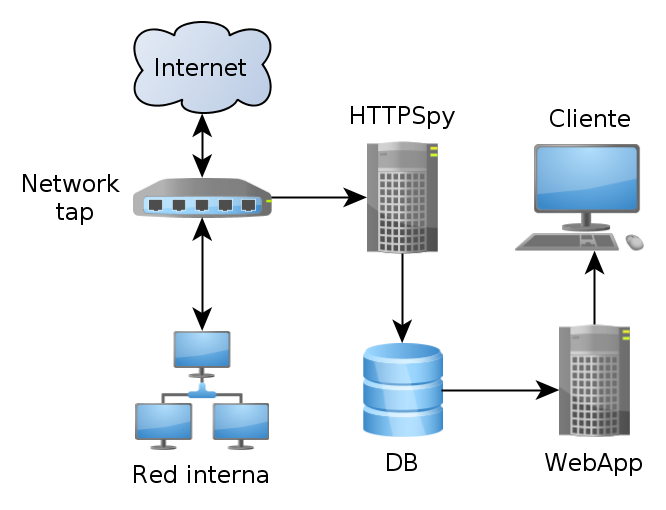
\includegraphics[scale=0.4]{img/deploy.png}
\end{figure}

Todo el tráfico que pasa entre la red interna e Internet debe pasar por el Network Tap (en nuestro caso un proxy) y allí es cuando ese tráfico es capturado por el sniffer que implementamos (HTTPSpy). El mismo si detecta paquetes pertenecientes al protocolo HTTP o HTTPS rearma dichos paquetes y los almacena en una base de datos para su posterior análisis. Finalmente, un usuario cliente puede ingresar a la aplicación web y realizar consultas sobre datos a partir de los registros capturados y almacenados en la base de datos por el sniffer.
Adicionalmente, aunque no está grafico, nuestro sniffer también puede conectarse con un servidor smtp y enviar un mail al cumplirse ciertas condiciones sobre las conexiones.
